\chapter{Estimation of Time-resolved Velocity Fields}
Analysis of the evolution and interaction of the large-scale structures, and ultimately the noise generated thereby, is greatly simplified by the acquisition of time-resolved flow-field measurements.
(In fact, as will be discussed in \sect{sect:source}, computation of the aeroacoustic source field will eventually require a temporal derivative and thus time-resolved data is a necessity for the current work.)
Unfortunately, directly acquiring time-resolved velocity fields for the jet currently under study is simply not possible due to the combination of a large domain of interest ($0 \leq z/D \lesssim 12, 0 \leq r/D \lesssim 3$) and high characteristic frequencies on the order of several kilohertz.
Full-field, high-fidelity measurement techniques capable of this repetition rate simply do not exist at present.
An indirect method is therefore required in order to estimate the evolution of the large-scale structures, in a reduced-order sense.

Phase-locking of a data acquisition system to actuators (or a naturally occurring resonance tone) is a common experimental technique; by varying the delay between the trigger and time of data acquisition, multiple phases can be acquired and the coherent component of the phenomena can be analyzed.
Phase-locking of the PIV system to the LAFPAs was initially considered for the present work, but quickly discarded.
Sample analysis performed using a numerical database indicated that a very high temporal resolution was required in order to accurately compute fluctuation rates in the dilatation field (the relevance of which will become more apparent in the following chapter).
At moderate to high excitation frequencies, this was feasible, though potentially tedious (for example, $\sim$16 phases were estimated as necessary at $St_{DF} =0.25$).
At $St_{DF} =0.05$ however, this would require roughly \textit{forty} phases (the significant dead time between actuations means that it is not necessary to acquire the entire range of phases from $0$ to $2\pi$, but this is small consolation).
Clearly, a more efficient data acquisition method is in order.
\section{Stochastic Estimation}
Stochastic estimation was first proposed by Adrian [cite 1977] in 1977, as an outgrowth from the conditional statistical analyses popular at the time. 
Large-scale coherent structures had been educed from anisotropic turbulent flows (such as boundary or shear layers) by conditional sampling techniques.
Adrian succeeded in identifying detailed flow structures (`conditional eddies') in isotropic turbulence by computing a mean-square estimate of the flow from linear two-point correlations (higher-order, nonlinear correlations were explored in Adrian [cite 1979]). 
The methodology was extended in Adrian [cite 1994] to estimation of velocity fields using spatial correlations coupled with a reduced set of measurements.

Stochastic estimation attracted considerable attention from the fluid dynamics community due to its potential to educe meaningful structures and behavior from highly turbulent, incoherent flows as well as its relative simplicity.
Subsequent researchers refined stochastic estimation in several important aspects.
Bonnet \etal [Bonnet1994] developed the complementary technique by combining linear stochastic estimation (LSE) with proper orthogonal decomposition (POD), improving the accuracy due to higher correlation levels between low-order modes.
The estimated velocity fields produced by LSE were projected onto the POD eigenfunctions (computed from the random, non-time-resolved velocity fields) to produce an estimate of the time-dependent POD coefficients, which can then be used to reconstruct low-order representations of the estimated random velocity field.
Picard \& Delville [Picard2000] used LSE and POD to link the longitudinal pressure distribution surrounding a low subsonic jet to vortical motions in the shear layer by simultaneously sampling microphone and hotwire data.
In Boree [Boree2003] the POD coefficients of the velocity field were estimated directly, using pressure modes.
Ewing \& Citriniti [Ewing1997] extended the standard form of LSE, in which spatial correlations are computed at a single time lag, by Fourier transforming the reference signal in time prior to computing the two-point cross-correlations (now cross-spectra). 
The incorporation of phase-delay information over a range of frequencies (and in essence, including information from multiple time lags) was found to significantly improve the accuracy of the reconstructions for many flow regimes [Ewing1997,Tinney2006,Tinney2008].
Finally, multi-time-delay LSE-POD was performed in the physical domain (as opposed to the Fourier) by Durgesh \& Naugton [Durgesh2010] to study the turbulent structures in a near wake region.

The current work borrows heavily from the methodology of Tinney \etal [TinneyJFM2008] and Sinha \etal [SinhaIJFC2010] in order to estimate the two-component time-resolved velocity field on a streamwise slice of the jet.
As explained in \sect{sect:piv_method}, two-component PIV snapshots were acquired at well-defined instants of near-field pressure traces.
The computational methodology by which the stochastic estimation is performed has been modified extensively, however.
???  
\subsection{Stochastic Estimation via Artificial Neural Networks}
Artificial neural networks (or simply, `neural networks'), are statistical computing models which developed as a branch of machine learning.
The design of neural networks is based on simplified models of the human brain: they are comprised of a large number of simple, connected computing cells (`neurons') and therefore are massively parallel distributed processors.
The neurons themselves are based on models of biological neurons, and produce a single output based on the linear summations of inputs (either directly from the user or from other, lower-level neurons) and synaptic weights which is then modulated by a nonlinear activation function.

\subsection{Phase-averaging versus Phase-locking}
\section{Large-Scale Structure Interactions}
\subsection{Time-Averaged Effects}
\begin{figure}
	\centering
	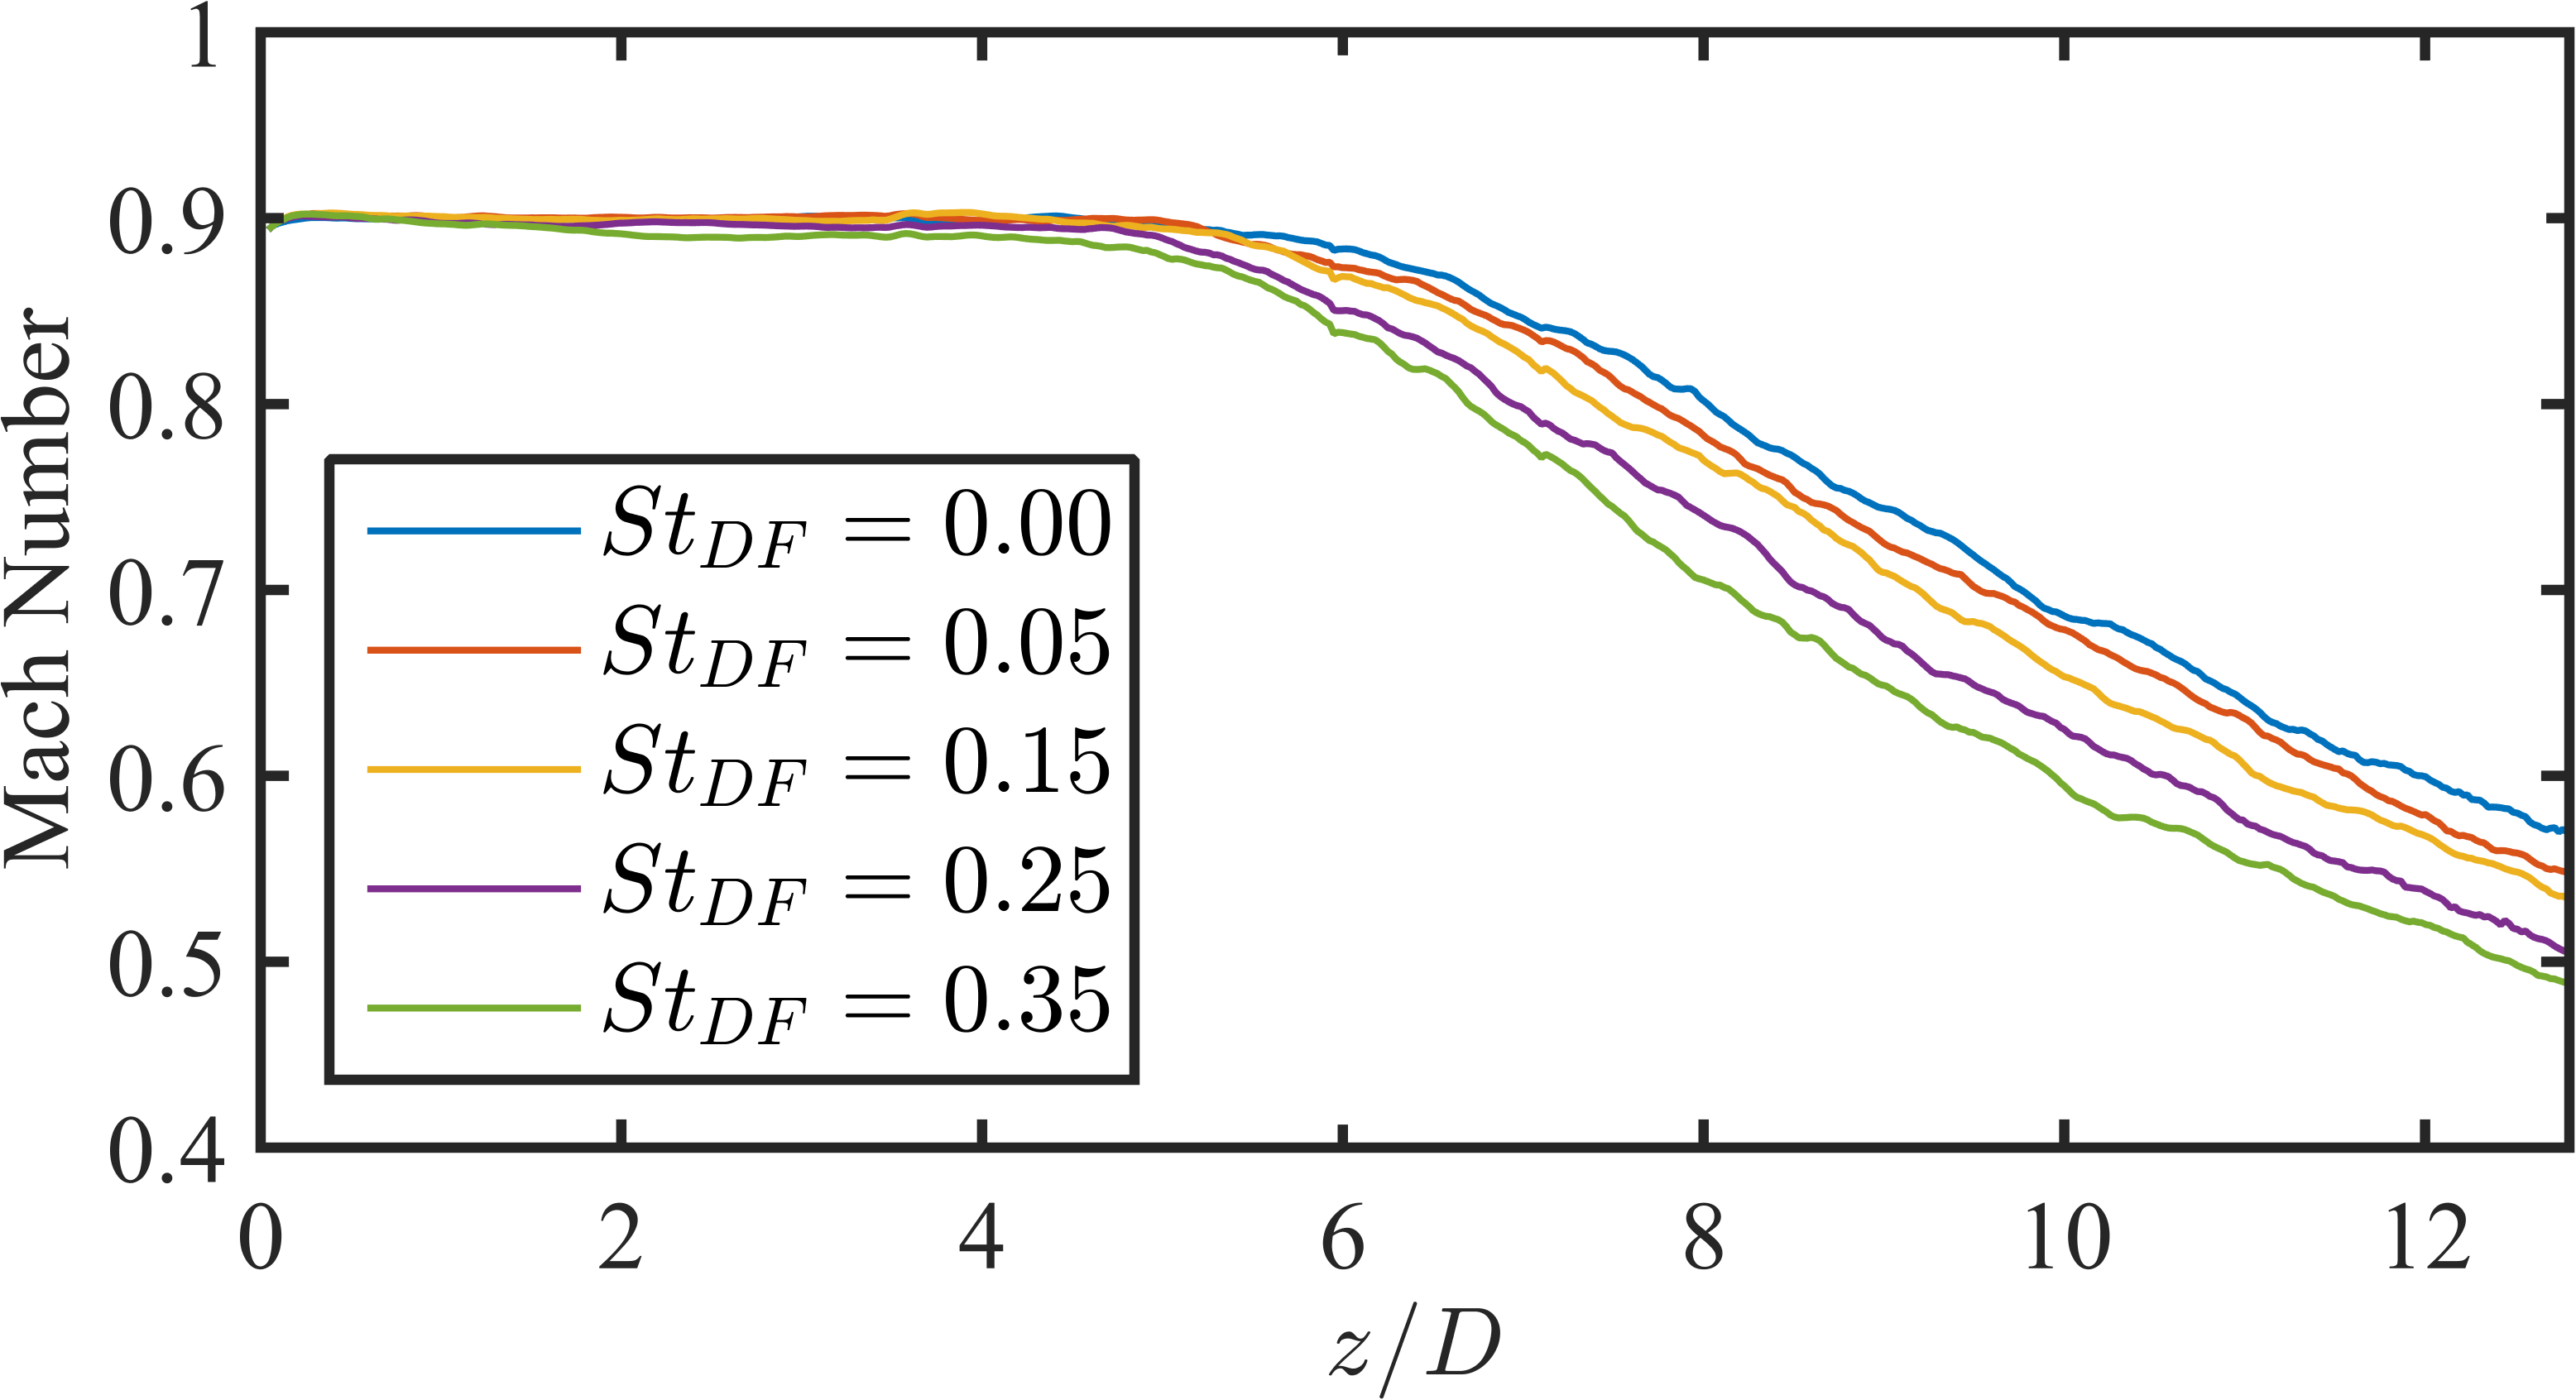
\includegraphics[width = 3.5in]{Figures/ch4_centerlineMach.png}
	\caption{Centerline Mach number for all excitation cases; baseline jet is indicated by `0.00'.}
	\label{fig:ch4_centerlinemach}
\end{figure}